\chapter{Mathematical Models of Identifying Sections}

\section{Data Analysis}
The following section describes the data used. To ensure that the data recorded via the accelerometer can be evaluated, modifications such as smoothing and noise filtering had to be made. These are described below. But first the used data model is shown.

\subsection{Data Model}
The used Model consists of four parameters:
\begin{itemize}
	\item \textbf{Round}: represents the current lap
	\item \textbf{Time Stamp}: represents the current time stamp for each step
	\item \textbf{X-Acceleration}: represents the force that indicates curves
	\item \textbf{Y-Acceleration}: represents the force that indicates the acceleration of the vehicle
\end{itemize}
The reason, why only the forces in x- and y-directions are used, is that the device lies flat on the vehicle. In this case the z-acceleration only indicates the force of gravity, which is not necessary for this work.\\
The round is not altered, therefore it will not be mentioned any further. 

For the initial data one entry containing the four parameters is taken every 10 milliseconds. Figure \ref{fig:origFor} shows the forces for one lap in the original data.

\begin{figure}[H]
	\centering
	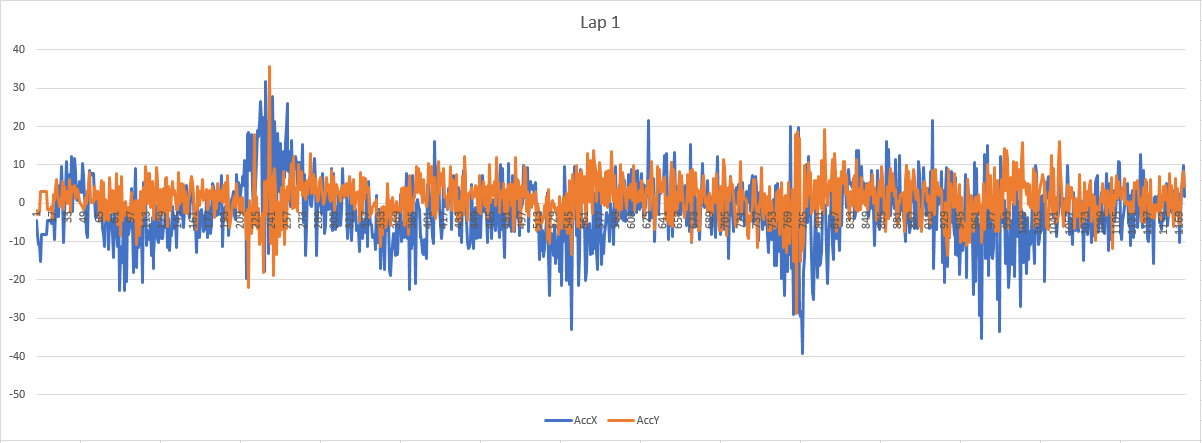
\includegraphics[scale= 0.42]{Pictures/originalForces.png}
	\caption{Visualization of the forces in the original data}
	\label{fig:origFor}
\end{figure}

This figure shows clearly that a analysis on base of the unfiltered data is simply impossible. Therefore as a first step data smoothing is used which is described in the following.

\subsection{Smoothing}
One problem that was identified is that there are to many measured points over time. So at first every four to five measured points were summed up and the average was used. This resulted in a better graph, which is shown in figure \ref{fig:smoFor}.

\begin{figure}[H]
	\centering
	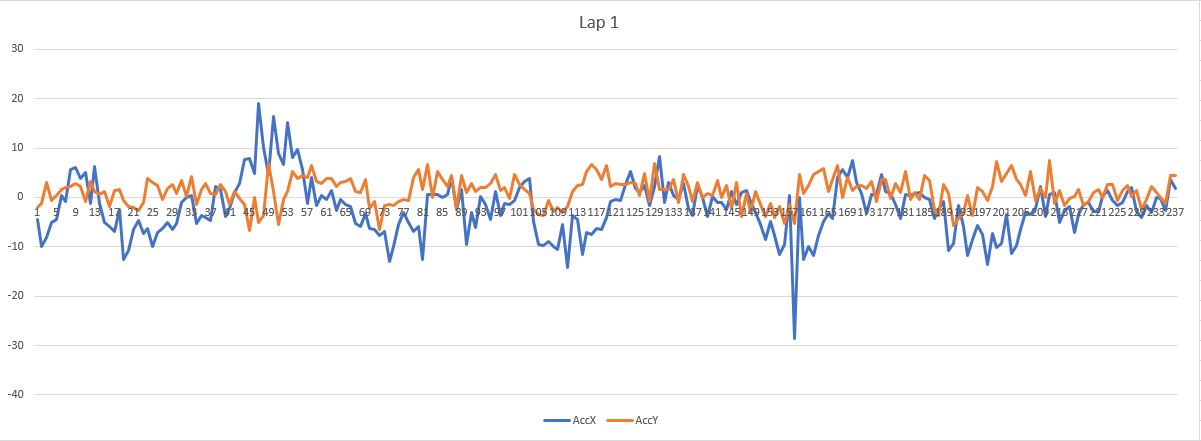
\includegraphics[scale= 0.45]{Pictures/smoothedForces.png}
	\caption{Visualization of the forces of the smoothed data}
	\label{fig:smoFor}
\end{figure}

In this figure it is possible for the human eye to distinguish between sections like left and right curves. But because of the noise, it would still be difficult for a computer. So a noise filter had to be used. It is described in the following section.

\subsection{Savitzky-Golay Filtering}
This filter is used to increase the signal-to-noise-ratio of a digital data set\cite{sg}. Therefore it would perfectly fit the requirement. It requires a data set consisting of $n$ points $(x,y)$ where x is an independent variable and y is the observed value. In this case $x$ is the time stamp, while $y$ is the force in x-/y- direction. In addition a set of $m$ convolution coefficients $C_i$ are needed which results in following equation:
\begin{equation*}
	Y_j = \sum_{i=-\frac{m-1}{2}}^{\frac{m-1}{2}}\dfrac{C_i\cdot y_{j+i}}{h},~~~~~~~ \dfrac{m-1}{2}\leq j \leq n-\dfrac{m-1}{2}
\end{equation*}
Because of the high sample rate in this project a relatively high value for $m=9$ was used. Therefore 9 convolution coefficients were used:
\begin{equation*}
	\begin{split}
	C_{-4} & = -21\\
	C_{-3} & = 14\\
	C_{-2} & = 39\\
	C_{-1} & = 54\\
	C_{0} & = 59   \\
	C_{1} & = 54     \\
	C_{2} & = 39     \\
	C_{3} & = 14     \\
	C_{4} & = -21    \\
	\end{split}
\end{equation*}
The sum of these coefficients is used for the normalisation $h=231$.

Applying this filter on the not smoothed original data results in a graph shown in figure \ref{fig:sgoriFor}.

\begin{figure}[H]
	\centering
	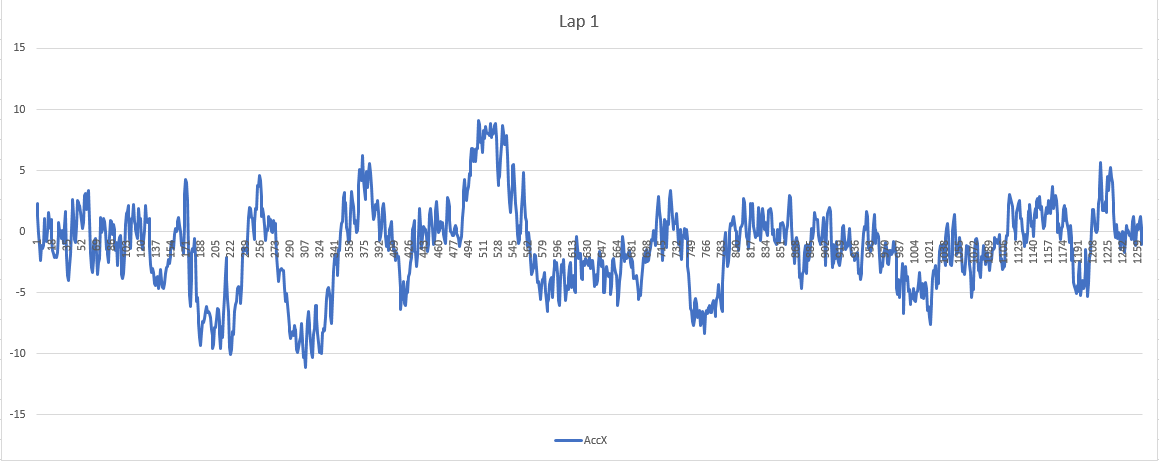
\includegraphics[scale= 0.45]{Pictures/sgoriForces.png}
	\caption{Visualization of the forces of the applied filter on the original data}
	\label{fig:sgoriFor}
\end{figure}

This proves, that a pre-smoothing might be needed to get a less noisy graph. Therefore figure \ref{fig:sgFor} shows the graph that is accomplished after applying both methods.

\begin{figure}[H]
	\centering
	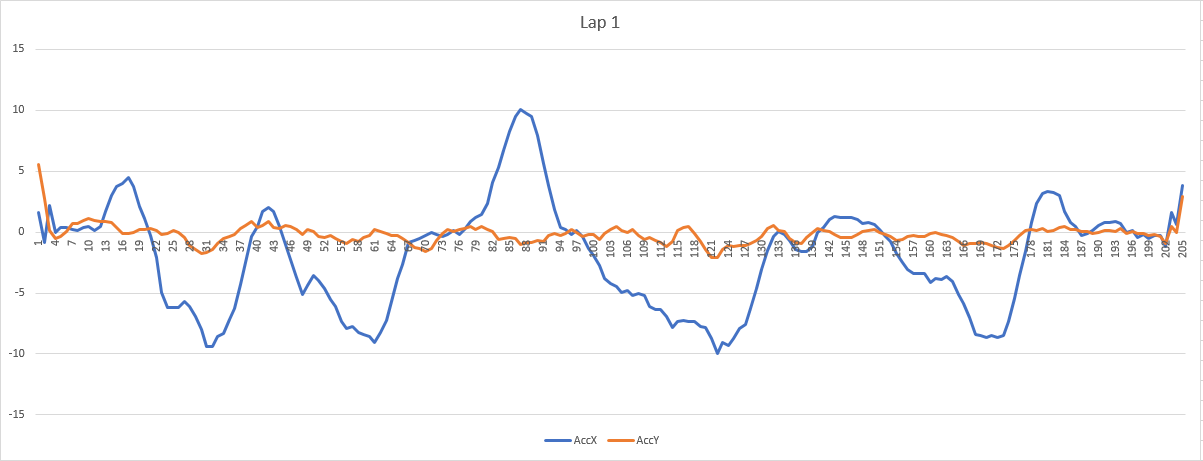
\includegraphics[scale= 0.45]{Pictures/sgForces.png}
	\caption{Visualization of the forces of the applied filter on the smoothed data}
	\label{fig:sgFor}
\end{figure}

With all this smoothing and filtering it is now possible for a computer to identify sections, which is described in the next section.

\newpage
\section{Section Identification}
The following section will describe the used solution for the identification and validation of sections. And is split into four parts. The first explains the rough identification of sections. These sections will then be given to a classification method that clearly identifies the type of section, be it a curve or a straight line. Afterwards the fitting of thresholds and lap validation will be explained. The last part contains the definition for the performance tips.

\subsection{Identification}\label{identification}
The identification is split into three parts that will be executed serial. After smoothing and filtering of the dataset. The x-axis acceleration values will be split into two groups. This split is happening with a singular x value representing a threshold called \code{CURVETHRESHOLD}. This threshold will be applied in the positive and negative acceleration range. A visual representation of the \code{CURVETHRESHOLD} can be seen in figure \ref{upperlowerBound}. In this graph, the threshold is set to 3.5. All points below the lower bound and above the upper bound will be grouped inside a dataset, while all the points in between are grouped in another.
\begin{figure}[H]
	\centering
	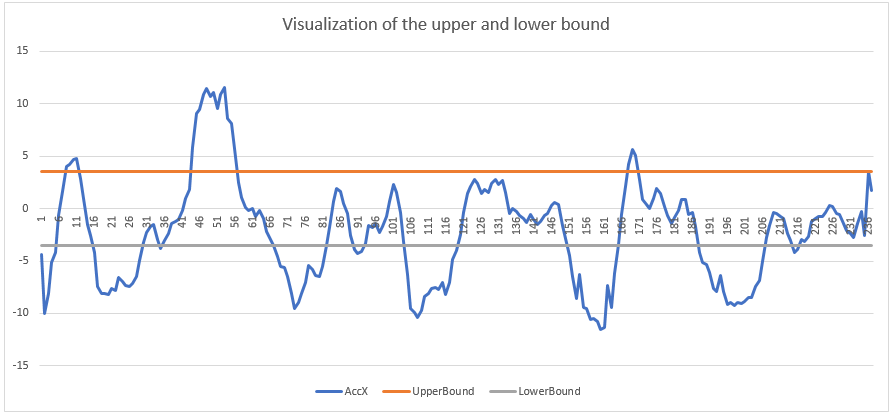
\includegraphics[scale= 0.6]{Pictures/upperandlowerbound.png}
	\caption{Visualization of the thresholds for the upper and lower dataset}
	\label{upperlowerBound}
\end{figure}
After separating the datasets with the threshold, the points above the \code{CURVETHRESHOLD} are considered as curves. Therefore it is cleaned in a second step. Because a curve cannot be created with only one point above the \code{CURVETHRESHOLD}, single points will be put back into the dataset in between the \code{CURVETHRESHOLD}. The last step is grouping the points into sections. The points in between are created as new sections with ten points. A section, that is above the threshold will be created with the first point above and the last point above. After creation of the section, the sections will be passed to the classification.

\subsection{Classification}\label{classification}
The classification works in multiple steps described in this section. At first each section in each lap is looked at closer. The following step needs three points of a section:
\begin{itemize}
	\item The x coordinate of the start ($s$)
	\item The x coordinate of the start ($e$)
	\item The y coordinate of the virtual median (acceleration on x-axis)
\end{itemize}

This is needed to determine a parabola for the section. A parabola can be represented by a function and therefore be integrated. The integral of the section is a significant help in identifying a section type. To specify the function of the parabola following equation is applied:

\begin{equation}
	f(x) = a (x-V)^2 + M
\end{equation}

where $V$ is the vertex of the parabola, or in this case the x-coordinate of the median, and $M$ is the y-coordinate of the median. The remaining unknown variable $a$ is calculated by:

\begin{equation}
a = \frac{M}{(s\cdot e) - \frac{(s+e)}{2}^2 }
\end{equation}

These equations are derived from the basic vertex form of parabolas by transformation of the equations. When the parabola function is established it is integrated to get the area enclosed by the parabola and the x-axis. This area is now used to classify sections. 

There is a range of thresholds to determine if an area is a curve or a straight section. The range of thresholds lies from 900 to 2500 and is iterated in steps of 100. When the area lies over the threshold, the section is identified as a right curve. If it is below the negative threshold the section identifies as a left curve. When the area is below the threshold the section is marked to be merged. The merging of sections is done until another curve is found. This way straight sections are not split into multiple parts.
\subsection{Validation and threshold fitting}
This section explains the applications process to validate the correct lap layout with the help of threshold fitting.

\subsubsection{Validation}
After the classification process, the resulting sections need to be validated, therefore a validation process is implemented. First, the lap needs to be chosen. This happens with considering all laps. The valid lap is the lap, with the most matching sections inside a lap. The process can be better described with the table visible in figure \ref{validation}
\begin{figure}[H]
	\centering
	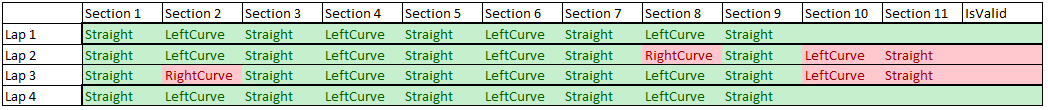
\includegraphics[scale= 0.5]{Pictures/validation.png}
	\caption{Table showcasing the validation process}
	\label{validation}
\end{figure}
Column one and four display exactly the same lap, while column two and three differ heavily from the first and fourth. Therefore we have two valid laps and two invalid laps, that will not receive a performance rating. These things can happen, if the driver takes the curve to hard and to long and needs to counter steer heavily outside the track. Therefore, an additional right curve is added inside the lap. We need to invalidate such laps, to provide a consistent result.
\newpage
\subsubsection{Threshold fitting}
To provide the best possible result, the \code{CURVETHRESHOLD} and the  \code{FORCETHRESHOLD} will be chosen in the analysis of the recorded laps. To provide the best result. The values that will be run are visible in Figure \ref{ThresholdValues}.
\begin{figure}[H]
\centering
	\begin{tabular}[c]{ l | l }
		Threshold & Values \\ \hline
		\code{CURVETHRESHOLD} & 900-2500 in 100 ticks \\
		\code{FORCETHRESHOLD} & 3-5 in 0.5 ticks \\
	\end{tabular}
\caption{Table for the threshold values}
\label{ThresholdValues}
\end{figure}
This fitting is needed, depending on the dataset. If the driver is rather cautious and drives slowly and steady through the track, the acceloremeter highs are way lower than if driven aggressively this can be seen in figure \ref{agressiveDriv}. It is clearly visible, that the aggressive dataset has highs way over ten, while the cautious dataset is always under ten.
\begin{figure}[H]
	\centering
	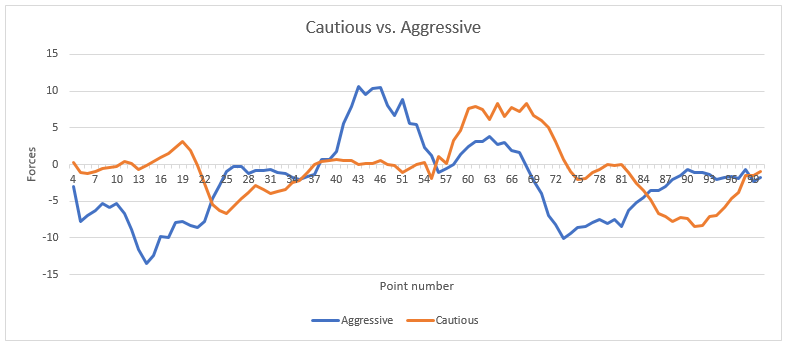
\includegraphics[scale= 0.6]{Pictures/agressiveDriv.png}
	\caption{Showing the difference of maximum values for the force in a curve, considering aggressive and cautious driving}
	\label{agressiveDriv}
\end{figure}
With this defined, it is clearly not possible to define a single threshold for all datasets. Therefeore the fitting takes place. Each of the values visible in figure \ref{ThresholdValues} will be executed, therefore the identification from section \ref{identification} and the classification explained in section \ref{classification} will be executed eighty five times for each of the possible \code{CURVETHRESHOLD} and \code{FORCETHRESHOLD} combinations. After running each of them, the validation will be done. It is determined and saved how many valid laps the dataset contains with the chosen thresholds. The threshold pair with the most valid laps, is then chosen as the best and displayed on the result screen.

\section{Section Rating}
Because the focus of our project was the identification of sections, the section rating part contains a simple implementation. The core principle is determining the fastest lap and comparing the time footprint of the other sections to the sections of the fastest lap. Because in our model, a straight is following on a curve and vice versa, the following mappings are created. Figure \ref{StraightResultMapping} shows the mapping for a straight and the timestamp configurations while figure \ref{CurveResultMapping} shows the same for the curve. The green and red markings are showing, if the current lap is faster(green) or slower(red) on the current section than the fastest lap, that is chosen as reference.
\begin{figure}[H]
	\centering
	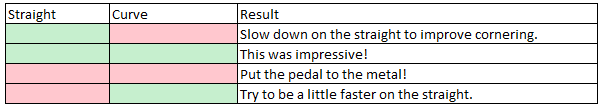
\includegraphics[scale= 0.9]{Pictures/StraightResultMapping.png}
	\caption{Mapping of the timestamps to the tips for a section, that is a straight}
	\label{StraightResultMapping}
\end{figure}

\begin{figure}[H]
	\centering
	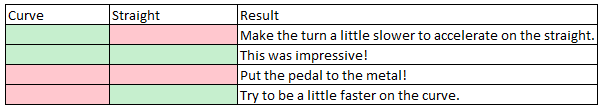
\includegraphics[scale= 0.9]{Pictures/CurveResultMapping.png}
	\caption{Mapping of the timestamps to the tips for a section, that is a curve}
	\label{CurveResultMapping}
\end{figure}
